\chapter{Proposed solution}\label{ch:proposed_solution}
\paragraph{}
We have picked SQM as the base for our algorithm. The main factors in this decision were that SQM is faster, produces smaller number of triangles, has better edge flow and even without smoothing the generated mesh better resembles the input skeleton. By avoiding the smoothing phase we do not need any input parameters to generate base mesh from an input skeleton. In this chapter we will explain each step of our proposed algorithm as well as extensions like elliptical nodes, cycles, etc.

\section{Skeleton straightening}\label{sec:straight}
Skeleton straightening is a preprocessing step that simplifies bridging of branch node polyhedrons. Straightened skeleton is a skeleton which nodes in every path between two branch nodes, two leaf nodes, or a branch node and a leaf node are co-linear. In addition we have added an extra condition that angles between child nodes of a branch node should be the same in straightened skeleton as they are in the input skeleton. To achieve the first condition for each connection node, we take the direction of a vector formed by connection nodes parents’ position and connection nodes position. The direction vector can be seen in Figure \ref{fig:straightening_ilu} as the green arrow. Then we normalize the direction vector and multiply it by the distance between connection node and its child node. The distance is marked by the black curve in Figure \ref{fig:straightening_ilu}. This vector represents the offset form connection nodes position at which lies the straightened position of its child node. We then calculate rotation between connection nodes child original position and its new position, in respect to the position of connection node. Finally, we rotate all descendants of the connection node. In order to conform to the second condition, at each branch node we do not alter the position of its child nodes.

\begin{figure}[h]
    \centering
    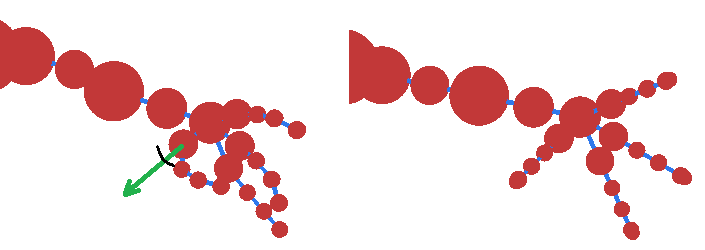
\includegraphics[width=\textwidth]{images/straightening2.png}
    \caption[Skeleton straightening]{Skeleton straightening. Left: input skeleton, green arrow represents the direction from connection nodes parents position to connection nodes position, black curve marks the distance between connection node and its child; right: straightened skeleton.}
    \label{fig:straightening_ilu}
\end{figure}

\subsection{Skinning}
In final vertex placement, we need to undo the rotations applied to the input skeleton during straightening. We have decided that the best solution is to use skinning since it can be implemented on GPU and we wanted to move all post-processing on the GPU. Straightened skeleton represents bind pose for skinning purposes and the input skeleton represents reference pose. Now we can calculate rotations, represented as quaternions, required to transform bind pose to reference pose. Traditionally, this would require to find the rotation between two corresponding nodes in respect to their parent. Rotating all child nodes in bind skeleton using the same rotation and propagate the rotation calculation to child nodes. However, since we know precisely how bind pose was constructed, we can exploit this knowledge and avoid the rotation of child nodes.
In fact, we do not even need the bind skeleton itself because the positions can be calculated from reference pose.

We want to calculate the rotation that would transform a node from its bind pose to its reference pose.
We know that the nodes parent is already in reference pose.
We also know that bind pose was constructed in such a way that all connection nodes child nodes are co-linear and preserve the distances between nodes.
That means from nodes parent reference pose we can calculate where would the node be in bind pose, if we would apply on it the same transformation matrices as were applied to its parent node.
The distance between parent and child nodes remains constant in both poses. And the direction at which the child node would be in bind pose is the same as the direction from its grandparent node to its parent node.
Now we only need to store the rotation between calculated child node position in bind pose and its actual position in reference pose with respect to its parent node.
The following algorithm demonstrates the calculation of a quaternion required to transform one node from straightened bind pose to input reference pose:
\begin{align*}
node& \leftarrow nodeInReferencePose \\
parent& = node.Parent \\
grandParent& = parent.parent \\
distance& = dist(node, parent) \\
direction& = normalize(parent - grandParent) \\
nodeInBind& = parent + distance * direction \\
u& = normalize(nodeInBind - parent) \\
v& = normalize(node - parent) \\
rotation& = QuaternionBetweenVectors(u, v)
\end{align*}



%In fact we do not even need the bind skeleton itself.
%
%This can be seen in Figure \ref{fig:DoF_estimation_ilu}. We want to calculate the rotation that would transform circle node to reference pose. We know that circle nodes parent square node is already in reference pose. We also know, that bind pose was constructed in such a way that all connection nodes childes are co-linear and preserve the distances between nodes. That means from squares reference pose we can calculate, where would be circle node, if we would apply on it the same transformation matrices as were applied to square node. The distance between square and circle node remains constant in both poses. And the direction at which the circle node would be is the same as the direction from triangle node to square node, which is marked as green arrow in Figure \ref{fig:DoF_estimation_ilu}. Now we only need to store the rotation between calculated circle node position, green circle in Figure \ref{fig:DoF_estimation_ilu} and its actual position red circle, with respect to its parent red square node.
%
%\begin{figure}[h]
%    \centering
%    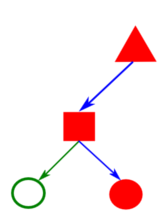
\includegraphics[height=6cm]{images/DoF_estimation.png}
%    \label{fig:DoF_estimation_ilu}
%    \caption[Rotation estimation from reference pose]{Rotation estimation from reference pose. Circle: node which rotation we want to estimate; Square: parent of circle node; Triangle: parent of square node; Blue arrows: edges in reference pose; Green circle: circle node position after applying squares skinning matrices; Green arrow: direction from square to green circle node;}
%\end{figure}

\section{BNP generation}\label{sec:bnp_gen}
For each branch node we calculate the direction from said branch node to each of its children and to its parent. Then we create rays with origin in branch nodes position and direction corresponding to the direction calculated previously. These rays can be seen in Figure \ref{fig:bnp_gen_ilu}a as blue arrows. We calculate the intersection of each of these rays with the sphere associated with the branch node. We store each intersection in a set of intersection points. Now we triangulate the intersection points. Different algorithms can be used to achieve the same effect, but we have picked Delaunay triangulation in spherical domain which was also used in the original paper. The algorithm works like standard Delaunay triangulation. With one exception, the predicate deciding whatever newly inserted triangle would lay in the circle of an already existing triangle is replaced. The new predicate compares angle between the newly inserted triangles normal with normals of already existing triangles. Result of triangulation is shown in Figure \ref{fig:bnp_gen_ilu}b as the blue triangle. We will use indexed face representation of the mesh, since that is the output of Delaunay triangulation. The generated polyhedron is now subdivided by inserting a point in the center of each face and in the middle of each edge. The vertex inserted in the center of each face is then connected with all vertices corresponding to the same face. So each triangle is subdivided into six smaller triangles. The newly inserted points are then projected onto the sphere associated with the node. The subdivision and projection is necessary because otherwise polyhedrons that would be generated with co-planar or nearly co-planar intersection points would have zero volume or very small volume, respectively. To project the newly inserted vertices onto the sphere, we once again use a ray-sphere intersection. The origin of the ray is the position of each newly inserted vertex. The direction of the ray is mean normal of the faces that are connected with the vertex. This means that for the vertices in the center of each face the normal of the subdivided face is used. For vertices inserted in the middle of each edge the mean normal of faces corresponding to that edge is used. Final polyhedron is shown in Figure \ref{fig:bnp_gen_ilu}c.

\begin{figure}[h]
    \centering
    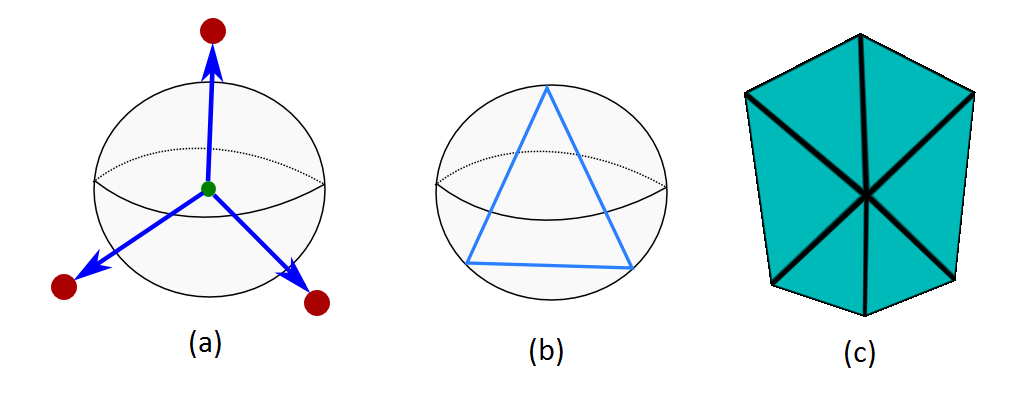
\includegraphics[width=\textwidth]{images/bnp_gen_ilu.png}
    \caption[BNP generation process]{BNP generation process. (a) green is a branch node, blue arrows represent direction vectors of rays, red circles represent child nodes; (b) blue triangle is the result of triangulation; (c) final subdivided BNP.}
    \label{fig:bnp_gen_ilu}
\end{figure}

Triangulation of intersection vertices can sometimes create obtuse triangles. These are problematic because when we insert the vertex in the middle of an obtuse triangle the one-rings of intersection vertices are not convex. If we would project the one-ring of the intersection vertex onto a plane, which is defined by the intersection point and the direction from skeletal nodes position to the intersection point, the resulting planar polygon would not be convex. In Figure \ref{fig:obtus_tri_ilu} we can see on the left how a polyhedron looks when it is generated with obtuse triangles. Expected central vertex position is marked by red arrow and expected edges are marked as yellow lines. This is not desirable since it would cause problems during cyclic mesh generation. To remedy this situation we calculate the projection of the central vertex in a different manner. The origin of the ray is the position of the vertex. But we use a new direction vector. This vector is the normal of a triangle formed by the projected points that were inserted in the middle of each edge. The result can be seen in Figure \ref{fig:obtus_tri_ilu} on the right.

\begin{figure}[h]
    \centering
    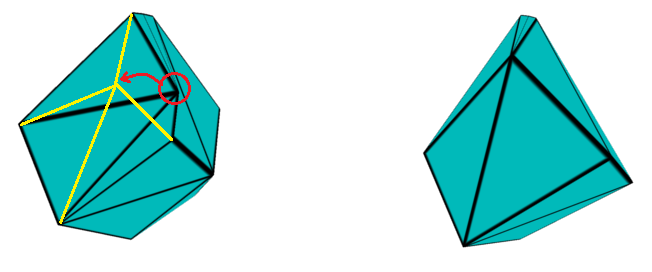
\includegraphics[height=4cm]{images/obtuse_triangle_fix_ilu.png}
    \caption[Obtuse triangle problem]{Obtuse triangle problem. Left: polyhedron with obtuse triangle. Red arrow marks vertex expected position and yellow lines mark expected edges; right: polyhedron after applying our fix.}
    \label{fig:obtus_tri_ilu}
\end{figure}

\section{BNP refinement}\label{sec:bnp_sub}
During the penultimate step of the algorithm, BNP joining, we want to connect two BNPs, with tube consisting solely from quadrilaterals. To ensure that we can use quadrilaterals only, we want intersection vertices connected via a path, to have the same number of nodes in their one-ring neighborhood. We take the notion of Link Intersection Edge (LIE) from \cite{sqm}. A LIE is a set of edges that are between vertices of two intersection vertices one-ring neighborhoods. In Figure \ref{fig:refinement_ilu}a one LIE is represented with yellow colored edges and a second LIE is represented with red colored edges. The refining of one BNP is a one-pass procedure. Since we will often need to access the one-ring neighborhood of a vertex, we convert our mesh to half-edge representation.

\paragraph{Preprocessing}
We start the refining of a BNP by creating a map of LIEs corresponding to each intersection vertex. For each intersection vertex, we store its corresponding LIEs, as well as the number of splits required by that vertex, to have the same valence as its corresponding vertex. An intersection vertex can be connected with three types of vertices. Each type defines how much we can split LIEs, corresponding to that intersection vertex.
\begin{itemize}
	\itemsep-0.25em 
	\item \textbf{Parents intersection vertex} - the number of splits is fixed. That is after splitting the valence of these two vertices must be exactly the same. This is necessary otherwise splits in child BNP could cause splits in parents BNP which could result in infinite loops.
	\item \textbf{Branch node intersection vertex} - difference between valencies of the two vertices is calculated. If the number is negative, that is corresponding vertex has smaller valence, we prefer not to split LIEs corresponding to current intersection vertex. If the number is positive, that is corresponding vertex has higher valence, we split LIEs corresponding to current intersection vertex so that the vertex has at least the same valence as its corresponding vertex.
	\item \textbf{Leaf node} - corresponding LIEs can be split as much as needed.
\end{itemize}

\begin{figure}[h]
    \centering
    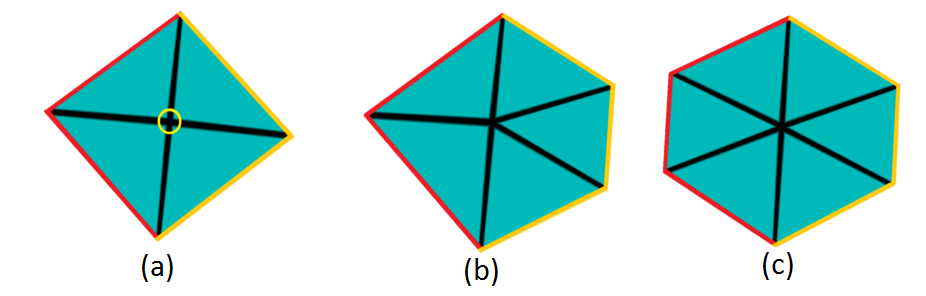
\includegraphics[width=\textwidth]{images/refinement_ilu.png}
    \caption[BNP refinement]{BNP refinement. Yellow edges represent Link Intersection Edge (LIE) corresponding to second intersection edge of the BNP. Red edges represent LIE corresponding to third intersection edge. Yellow circle marks the first intersection vertex. (a) BNP before subdivision; (b) BNP after one subdivision and one smoothing step; (c) final BNP after two subdivisions and two smoothing steps.}
    \label{fig:refinement_ilu}
\end{figure}

\paragraph{Subdivision}
We loop through all intersection vertices, starting with the intersection vertex connected with parents BNP and continuing with the rest. In each cycle, we split LIEs corresponding to current intersection vertex, until the valence of the intersection vertex is equal to its required number of splits. Every time we want to split a LIE we heuristically select the best based on two filters. The first filter is the splitting required by the other intersection vertex belonging to the same LIE. If two or more LIEs require the same number of splits we use a second filter. This filter picks the LIE that was split the least. When we are splitting a LIE, we always split a representative edge which is the first edge of the LIE. Because of that we need to apply a smoothing scheme to roughly equalize the lengths of edges in a LIE. 

The whole process can be seen in Figure \ref{fig:refinement_ilu}. In Figure \ref{fig:refinement_ilu}a the yellow circle marks an intersection vertex that needs to be split twice. Yellow edges represent a LIE corresponding to second intersection vertex and red edges represent a LIE corresponding to third intersection vertex. Both LIEs have the same need to be split and none of them was split previously. For the first split the yellow LIE is selected subdivided once and smoothed. The result of the first split is shown in Figure \ref{fig:refinement_ilu}b. For the second split the need of both LIEs is still the same. But yellow LIE was already split so this time the red LIE is selected, subdivided, and smoothed. Final refined BNP is shown in Figure \ref{fig:refinement_ilu}c.

\subsection{Smoothing}
Since we always split only one representative edge of a LIE we are applying a smoothing scheme to equalize the length of edges in a subdivided LIE. The smoothing is very important because generated base mesh quality directly depends on the selected smoothing scheme. Ideally, the length of each edge in a smoothed LIE would be equal. However, since smoothing is applied after every subdivision the smoothing algorithm should be reasonably fast. We propose four smoothing schemes. These smoothing schemes are illustrated in Figure \ref{fig:smoothing_ilu} where the polyhedron from Figure \ref{fig:refinement_ilu}a is subdivided twice and then smoothed with various smoothing schemes.

\paragraph{Averaging smoothing}
New position for each vertex on a LIE is calculated by averaging one-ring neighborhood corresponding to the vertex. We start with the last vertex of a LIE that is the vertex on the last edge of a LIE and move towards the first vertex. We move each vertex, except the first and the last vertices, to the barycenter of its one-ring neighborhood and project them back onto the sphere corresponding to BNPs node. The resulting smoothed polyhedron is shown in Figure \ref{fig:smoothing_ilu}a. This approach is iterative and would need several iteration to achieve global optimum. However, we have found that one iteration is enough for our needs.

\paragraph{Quaternion smoothing}
For each LIE we calculate a quaternion representing the rotation from the first vertex of the LIE to the last vertex of the LIE. From each quaternion we extract its corresponding axis of rotation and angle of rotation. We smooth only points between the first and the last vertex so the calculated axis of rotation and angle are constant. During each smoothing step we first count the number of vertices in a LIE. Then we divide the angle of rotation by that number and form a new quaternion from already calculated axis of rotation and the newly calculated angle. For each vertex in a LIE between first and last we apply the rotation stored in the quaternion and update its position. This method produces LIEs that lie on small circles of their corresponding sphere. The spacing between vertices is regular and thus its very suitable for our needs. The result of quaternion smoothing is shown in Figure \ref{fig:smoothing_ilu}b.

\paragraph{Area weighted Laplacian}
For Laplacian smoothing we have adapted the algorithm described in \cite{laplac}. The weights used for smoothing are based on the one-ring area of each vertex. We use one iteration of Laplacian smoothing and then project the new vertices back onto their corresponding sphere. The result is shown in Figure \ref{fig:smoothing_ilu}c. The result is usable since the edges have better distributed length, than without smoothing. However, averaging and quaternion smoothing produce results of better quality.

\begin{figure}[h]
    \centering
    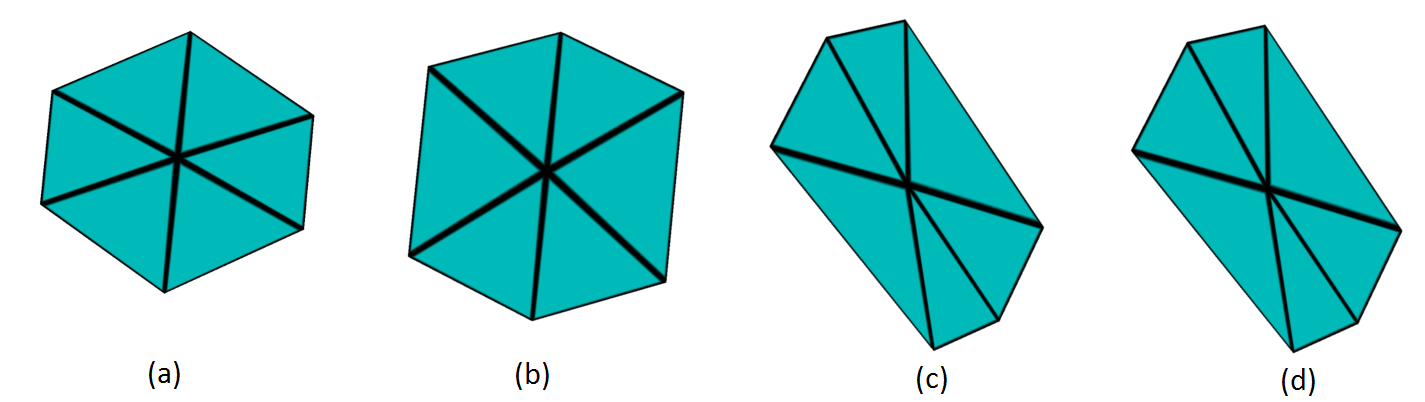
\includegraphics[width=\textwidth]{images/smoothing_ilu.png}
    \caption[LIE smoothing schemes]{LIE smoothing schemes. Shows results after applying: (a) averaging smoothing; (b) quaternion smoothing; (c) area weighted Laplacian smoothing; (d) valence weighted Laplacian smoothing.}
    \label{fig:smoothing_ilu}
\end{figure}

\paragraph{valence weighted Laplacian}
We use the same algorithm as for area weighted Laplacian with different contraction weights. The weights depend on the valence of each vertex. After Laplacian smoothing vertices are projected back onto their corresponding sphere. The result of this smoothing is very similar to area weighted Laplacian and is shown in Figure \ref{fig:smoothing_ilu}d.

\section{BNP joining}\label{sec:bnp_join}
After refinement of BNPs intersection vertices connected via path have the same valence. Now BNPs can be joined by tubes consisting from quadrilaterals only. We loop through each branch node in a depth-first search from skeletons root. We process each BNP in the following manner. We start with the whole BNP Figure \ref{fig:joining_process_ilu}a. We loop through all intersection vertices corresponding to current BNP. We remove each intersection vertex and its corresponding faces and edges from current BNP. In Figure \ref{fig:joining_process_ilu}b we can see the removal of third intersection vertex after first and second intersection vertices were joined. After the removal of an intersection vertex we continue joining all nodes on the path that produced the removed intersection vertex. We take the vertices forming the former one-ring of the removed intersection vertex. For each connection node on the path we duplicate the one-ring vertices, translate them to the nodes position and project them onto the sphere associated with the connection node. For the translation we construct a plane. The origin of the plane is the position of the connection node. The normal is the vector from the branch node to the connection node. Each vertex is translated along the normal until it lies on the plane. The projection is done by normalizing the vector from connection nodes position to each vertex and multiplying it by the radius of connection nodes corresponding sphere. These new vertices are then connected with previous set of vertices with faces and they are passed as current one-ring vertices for joining. In Figure \ref{fig:joining_process_ilu}c, we can see the translated connection node vertices before projection was applied. In Figure \ref{fig:joining_process_ilu}d the duplicated one-ring vertices are projected onto their associated sphere. After going through all connection nodes we can end either in a branch node or in a leaf node.

\begin{figure}[h]
    \centering
    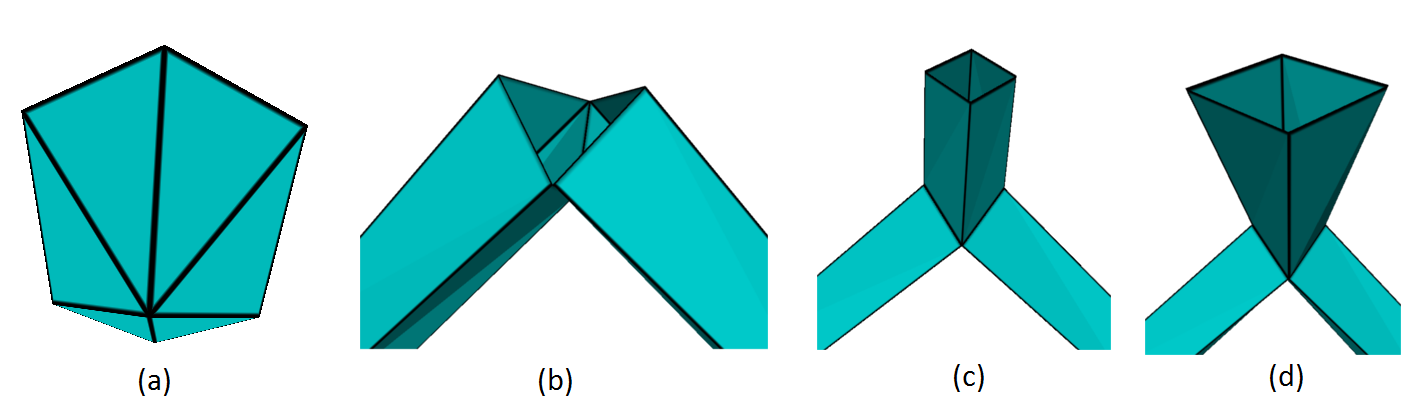
\includegraphics[width=\textwidth]{images/joining_ilu.png}
    \caption[BNP joining process]{BNP joining process. (a) polyhedron before joining; (b) polyhedron with removed faces corresponding to an intersection vertex; (c) new vertices for connection node before projection; (d) projected vertices of connection node.}
    \label{fig:joining_process_ilu}
\end{figure}

\paragraph{Branch node termination}
We start by removing the destination branch node corresponding intersection vertex and faces and edges connected to it. The tube generated from connection nodes should be joined with destination intersection vertex former one-ring. For this we need to find two corresponding vertices, which would form the first pair and define the pairing of the rest of the vertices. We can use multiple methods to find the first pair. The choice of the method affect output base mesh quality, as a wrong selection can lead into twists in the base mesh. We tested three methods.
\begin{itemize}
	\itemsep-0.25em 
	\item \textbf{Minimal Euclidean distance} - An arbitrary vertex is selected from current one-ring and its Euclidean distance to each vertex of destination one-ring is calculated. We match the vertex with the closest one. The main disadvantage of this method is that it is greedy end ends in local minima. That is to have the best overall mesh quality a more distant vertex would be a better choice. This can be seen in Figure \ref{fig:join_pairing_ilu}a where some connecting faces are twisted.
	\item \textbf{Minimal angle} - An arbitrary vertex is selected from the current one-ring. The direction from the selected vertex to each vertex of destination one-ring is calculated. Then we calculate the angle between this direction and the direction from original branch node to destination branch node. As a match we pick a vertex where the calculated angle was minimal. As before this method is greedy and can fall into local minima. An example of this is shown in Figure \ref{fig:join_pairing_ilu}b where some faces connecting the hand are twisted.
	\item \textbf{Minimal total Euclidean distance} - An arbitrary vertex is selected from current one-ring. We pair the vertex with each vertex of destination one-ring. Each pair defines a different mapping from the current one-ring vertices to destination one-ring vertices. We calculate the Euclidean distance between all paired vertices and store it as total Euclidean distance. Then we pick as pair the vertex where the total distance was minimal. The disadvantage of this approach is that it takes longer to compute. The advantage is that this approach avoids local minima by testing all the possible solutions and picking the best one. Since one-rings usually consist of few vertices we have decided to use this method. The resulting mesh using this pairing is shown in Figure \ref{fig:join_pairing_ilu}c. Among the possible results in Figure \ref{fig:join_pairing_ilu}c has minimal twisting compared to Figure \ref{fig:join_pairing_ilu}a and Figure \ref{fig:join_pairing_ilu}b. 
\end{itemize}

When the pairing of vertices is defined new edges can be formed between each pair and connect the geometry.

\begin{figure}[h]
    \centering
    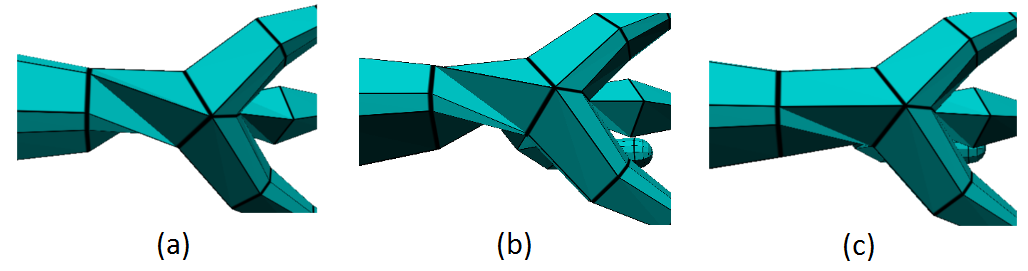
\includegraphics[width=\textwidth]{images/join_pairing.png}
    \caption[BNP joining pairing]{BNP joining pairing. (a) minimal Euclidean distance; (b) minimal angle; (c) minimal total Euclidean distance.}
    \label{fig:join_pairing_ilu}
\end{figure}

\paragraph{Leaf node termination}
As in original paper \cite{sqm} we have decided to terminate leaf nodes with triangular faces. Each face has two vertices from the current one-ring and one vertex is the position of the leaf node.

\section{Final vertex placement}\label{sec:fvp}
We use quaternions calculated during skeleton straightening.
For each skeletal node we accumulate the final rotation in a matrix.
Matrices are used because they are more suitable for GPU calculations than quaternions.
Linear blend skinning, as described in \cite{Kavan-07-SDQ}, is used to combine skinning matrices corresponding to each vertex on GPU.
We apply skinning transformation on GPU in vertex or tessellation shaders.
We have also implemented linear blend skinning on CPU.
This is advantageous for comparison purposes as well as when we are generating base meshes from cyclic skeletons.
Since we are using triangulations on CPU to close generate cyclic skeletons, we need to apply linear blend skinning before the triangulations.
Skinning could be still calculated on GPU and the resulting geometry could be send back to CPU for processing. However, we have found that our generated base meshes are relatively simple and the overhead from transmitting data between CPU and GPU would be more time consuming than CPU implementation of linear blend skinning.

\section{Ellipsoid Nodes}
An ellipsoid can be defined as a sphere with associated transformation matrix.
We take advantage of this representation of ellipsoids.
Instead of more complex ray-ellipsoid intersection that would have to be computed at each ellipsoid node, we have decided to represent each ellipsoid node as a sphere and a transformation matrix.
First our base mesh algorithm is evaluated as described previously with spherical nodes.
After that we send the transformation matrices corresponding to each ellipsoid node to GPU.
The vertices corresponding to each ellipsoid node are transformed directly in vertex shader.
Thanks to this, ellipsoid nodes require minimal extra computing resources from CPU.
The results can be seen in Figure \ref{fig:ellipsoid_ilu}.

\begin{figure}[ht]
    \centering
    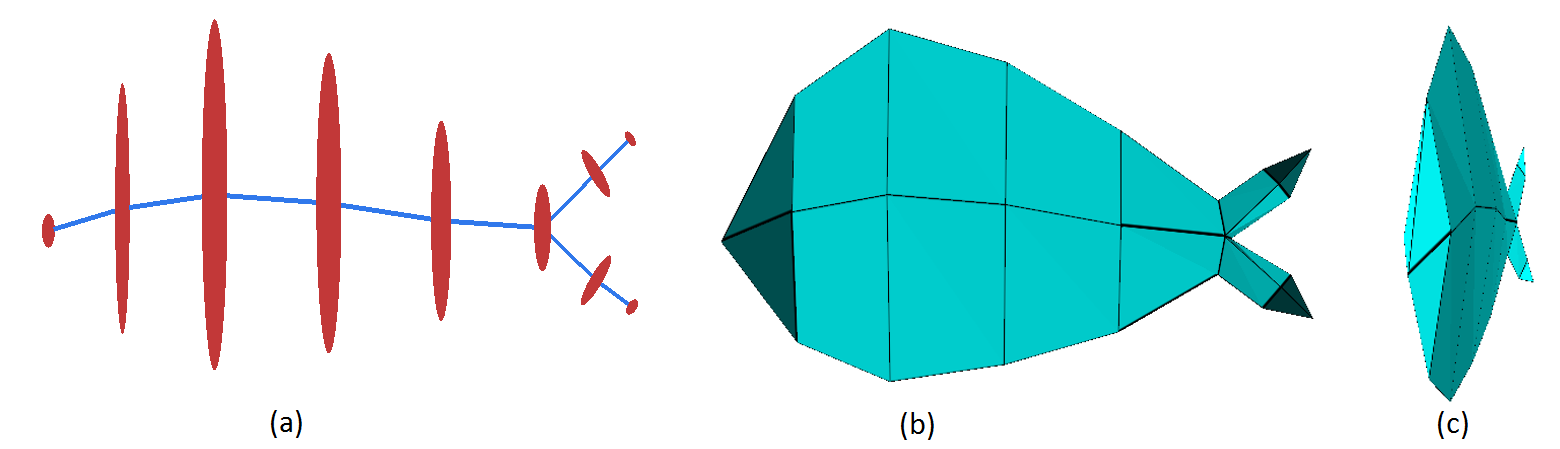
\includegraphics[width=\linewidth]{images/ellipsoid_fish_ilu}
    \caption[Ellipsoid nodes]{Ellipsoid nodes. (a) skeleton with ellipsoid nodes specified; (b) base mesh generated from skeleton; (c) base mesh from different angle.}
    \label{fig:ellipsoid_ilu}
\end{figure}

\section{Tessellation}
Tessellation shaders available since OpenGL 4.0 are used to tessellate the generated base mesh.
Two connected spherical nodes, a parent and a child, implicitly define a truncated cone between them.
The base of the cone has the radius of parent spherical node and the top of the truncated cone has the radius of child spherical node.
Each vertex generated during tessellation is projected onto this cone.
The projection is done by translating the vertex along its normal until it reaches the surfaces of the cone.
Tessellation is shown in Figure \ref{fig:tessellation_ilu}, the generated base mesh is shown in Figure \ref{fig:tessellation_ilu}a and the tessellated base mesh in Figure \ref{fig:tessellation_ilu}b.
However, during this step the generated base mesh gains volume and the newly generated vertices can intersect the tessellated base mesh.
This effect can be seen in Figure \ref{fig:tessellation_ilu}c.
To recover from this situation, we detect sharp vertices in the input mesh and apply a radius scaling scheme.
Sharp vertices are vertices which faces are forming acute angles.
In tessellation shader we have access only to one patch and its vertices.
So we compute the sharpness of each vertex by comparing and thresholding the normal of each vertex with the normal of the patch.
The smaller the angle between vertex normal and patch direction is, the sharper the vertex is.
We apply Bezier curves to modify the radius of the truncated cone.
We use Bezier curves that yield values between $[0;1]$.
For each tessellated vertex its distance from the beginning of the patch is calculated.
The distance is equal to tessellation parameter $v$ computed by the GPU.
Scaling reduction factor is calculated by sampling a point on Bezier curve at point $t = distance$.
The radius of each vertex is then multiplied with calculated factor.
The smoothed mesh is shown in Figure \ref{fig:tessellation_ilu}d.
Currently, the scaling Bezier curve is constant but it could be dynamically changed based on the sharpness of the vertices.

\begin{figure}[ht]
    \centering
    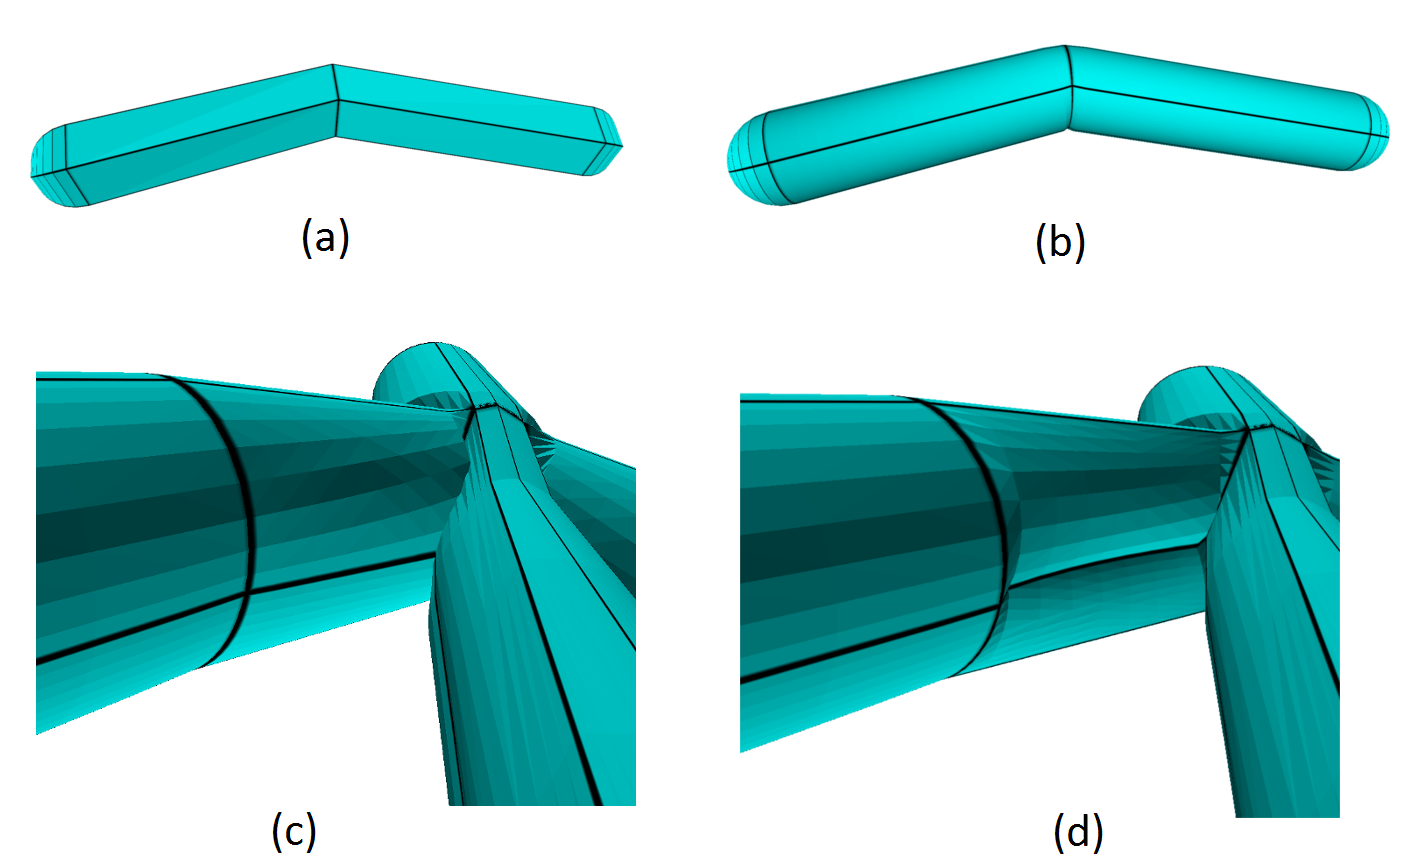
\includegraphics[width=0.9\linewidth]{images/tess_ilu}
    \caption[Tessellation and smoothing]{Tessellation. (a) non-tessellated mesh; (b) tessellated mesh wit 20 subdivisions; (c) tessellated mesh with self intersection; (d) tessellated mesh with radius scaling reduction.}
    \label{fig:tessellation_ilu}
\end{figure}

\section{Capsule Ending}
A capsule is a hemisphere generated at each leaf node of the input skeleton.
This hemisphere replaces the triangle fan pyramid generated by original SQM algorithm.
Generating of capsules can be approached in two ways.
The first is to generate a capsule at each leaf node corresponding to its radius.
The second is inserting additional nodes into the input skeleton with decreasing radius that would approximate a capsule.
We have implemented the second approach because it fits nicely into our pipeline.
Capsules generated this way can be directly tessellated on the GPU without any additional processing.
At each capsule leaf node, we insert additional nodes into the input skeleton proportional to the radius of the capsule node.
The radius of each node is decreased according to Equation \ref{eq:radius_change} where $nodeRadius$ is the radius of capsule node and $step$ is a number between $(0-1]$, that represents the distance from center of the capsule to its edge.
Final tessellated capsule is shown in Figure \ref{fig:capsule_ilu}.

\begin{equation}
newRadius = \sqrt{nodeRadius^{2} * (1 - step^{2})}
\label{eq:radius_change}
\end{equation}

\begin{figure}[ht]
    \centering
    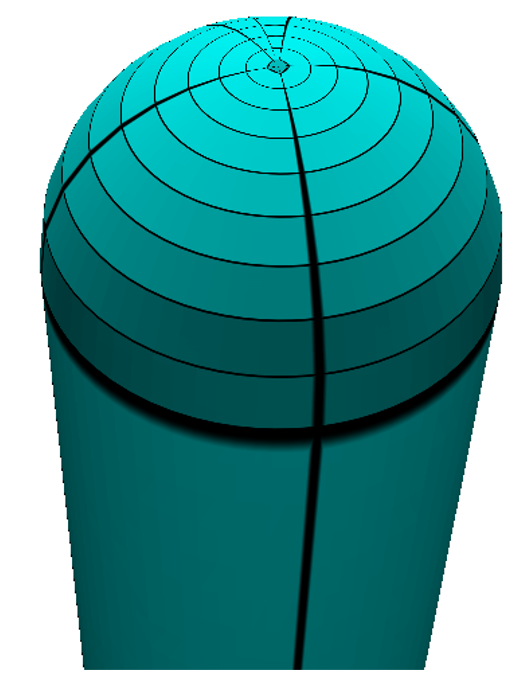
\includegraphics[width=0.5\textwidth]{images/capsule}
    \caption[Capsule generation]{Capsule generated by our algorithm and tessellated on GPU in tessellation shaders.}
    \label{fig:capsule_ilu}
\end{figure}

\section{Linear Skeletons}
Linear skeletons without branch nodes lack the initial geometry that is generated during BNP generation step described in Section~\ref{sec:bnp_gen}.
Additional nodes could be inserted into the input skeleton to form at least one branch node but we have found that it needlessly disturbs the flow of the output mesh.
Instead we decided to use a different approach.
We introduce an additional input parameter $N$ which specifies how many vertices should be generated for each node of the linear skeleton.
This parameter does not decrease the robustness of our approach, because additional vertices are generated during tessellation and the original number of vertices is negligible.

First step of the algorithm is setting the root to be the head of the input linear skeleton.
Next step of the algorithm is straightening of the input linear skeleton.
The input skeleton is shown in Figure \ref{fig:worm_ilu}a.
Next, $N$ vertices are generated around first connection node which is a child of the root node.
These vertices are distributed regularly around the node by slerping a quaternion which center of rotation is nodes position, axis of rotation is the direction from connection node to root node and magnitude is $360/N$.
Newly generated vertices are then joined with other vertices as in original base mesh algorithm.
Leaf nodes form a triangle fan and connection nodes form a tube of quadrilaterals.
The joined linear base mesh is shown in Figure \ref{fig:worm_ilu}b.
Skinning matrices are used to transform the generated linear skeleton into its input pose Figure \ref{fig:worm_ilu}c.

\begin{figure}[ht]
    \centering
    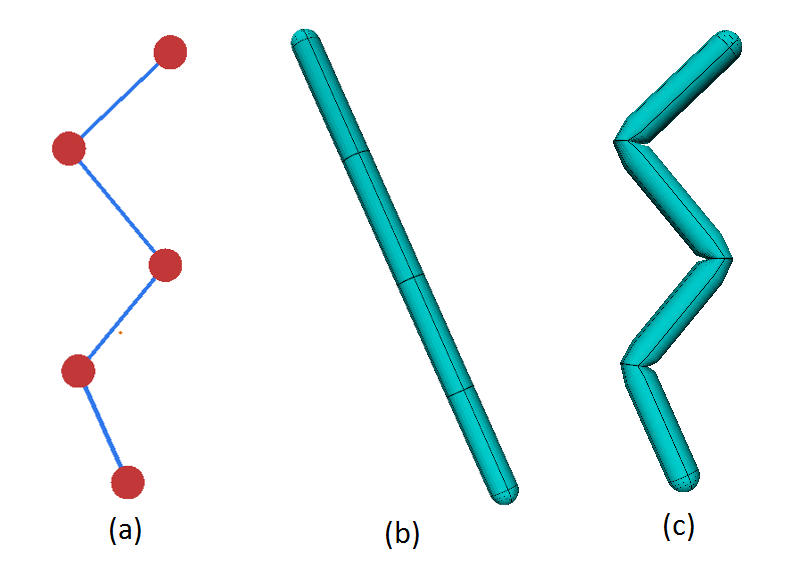
\includegraphics[width=0.7\textwidth]{images/worm_generation}
    \caption[Linear base mesh]{Linear base mesh generation. (a) input linear skeleton; (b) straightened and joined linear skeleton; (c) final linear base mesh.}
    \label{fig:worm_ilu}
\end{figure}

\section{Root That Is Not a Branch Node}
If the root of the input skeleton is not a branch node and a branch node is present in the skeleton, we can find it with a depth first search.
When we have at least one branch node we can re-root the tree so that the located branch node would be the root of the tree.
We apply Algorithm \ref{alg:reroot} to re-root the skeleton.
We want to make the input node the root of the skeleton.
For that it has to have no parent node and all other nodes in the skeleton should have a parent node.
We set the new root to have no parent and store its former parent as $current$ node and the parent of $current$ node as $currentParent$ node.
In a loop we set $currentParent$ as a child of $current$ node.
In order to advance along the skeleton, we set $current$ node to the parent of $current$ node and $currentParent$ node to the parent of $currentParent$ node.
This way we ascend along the skeleton, until we reach the former root node and the algorithm terminates.
\begin{algorithm}[h]
\caption{ReRoot}
\label{alg:reroot}
\begin{algorithmic}
	\STATE{\textbf{Input:} $node$}\COMMENT{the node that should be the new root}
	\STATE{$current \leftarrow node.parent$}
	\STATE{$currentParent \leftarrow current.parent$}
	\STATE{$node.parent \leftarrow NULL$}
	\STATE{$current.parent \leftarrow node$}
	\STATE{$current.removeChild(node)$}
	\STATE{$node.addChild(current)$}

	\WHILE{$current \neq root$}
		\STATE{$current.addChild(currentParent)$}
		\STATE{$parent.removeChild(current)$}
		\STATE{$newParent \leftarrow currentParent.parent$}
		\STATE{$currentParent.parent \leftarrow current$}
		\STATE{$current \leftarrow currentParent$}
		\STATE{$currentParent \leftarrow newParent$}
	\ENDWHILE
	\STATE{$root = node$}
\end{algorithmic}
\end{algorithm}

\section{Cyclic Skeletons}
Our last improvement is generation of base meshes from cyclic skeletons.
The cycle can be placed anywhere in the input skeleton.
The base algorithm could not be modified to allow generation of cyclic meshes because during BNP refinement step of the algorithm a cycle could cause an infinite loop.
However, we can modify the input skeleton in a way that would allow us to generate cyclic skeletons.
As the input we have a cyclic skeleton Figure \ref{fig:cycle_skeleton}.
Cyclic edge is marked with yellow color and cyclic nodes with green and violet colors.

First, we split the cycle by removing the yellow cyclic edge.
To each cyclic node we add an extra child node as shown in Figure \ref{fig:cycle_break}.
Light green node for green cyclic node and pink node for violet cyclic node.
These new nodes serve to preserve the skinning matrices that will rotate tubes generated from cyclic nodes to face each other. This can be seen in Figure \ref{fig:cycle_before}. Base mesh was generated as described in Chapter \ref{ch:proposed_solution} with one exception.
The triangles that should been generated for light green and pink nodes were omitted.
Now the gap between cyclic nodes can be closed.
We first project vertices associated to each cyclic node to a plane with origin at $O(0, 0, 0)$ and normal $n(0, 1, 0)$.
Next, we normalize the vertices so that vertices associated with violet node lie at a circumference with radius 1 and vertices associated with green node lie at circumference with radius 2.
The position of projected points is shown in Figure \ref{fig:cycle_del_before} where vertices associated with green node have green color and vertices associated with violet node have violet color.
Now we execute a Delaunay triangulation on the transformed points.
After the triangulation is done, we exclude triangles generated solely between green or violet vertices.
The remaining triangles represent the faces that should be generated in order to close the gap between cyclic nodes as can be seen in Figure \ref{fig:cycle_del_after}.
Final cyclic mesh is shown in Figure \ref{fig:cycle_after}.

%\begin{figure}[ht]
%    \centering
%    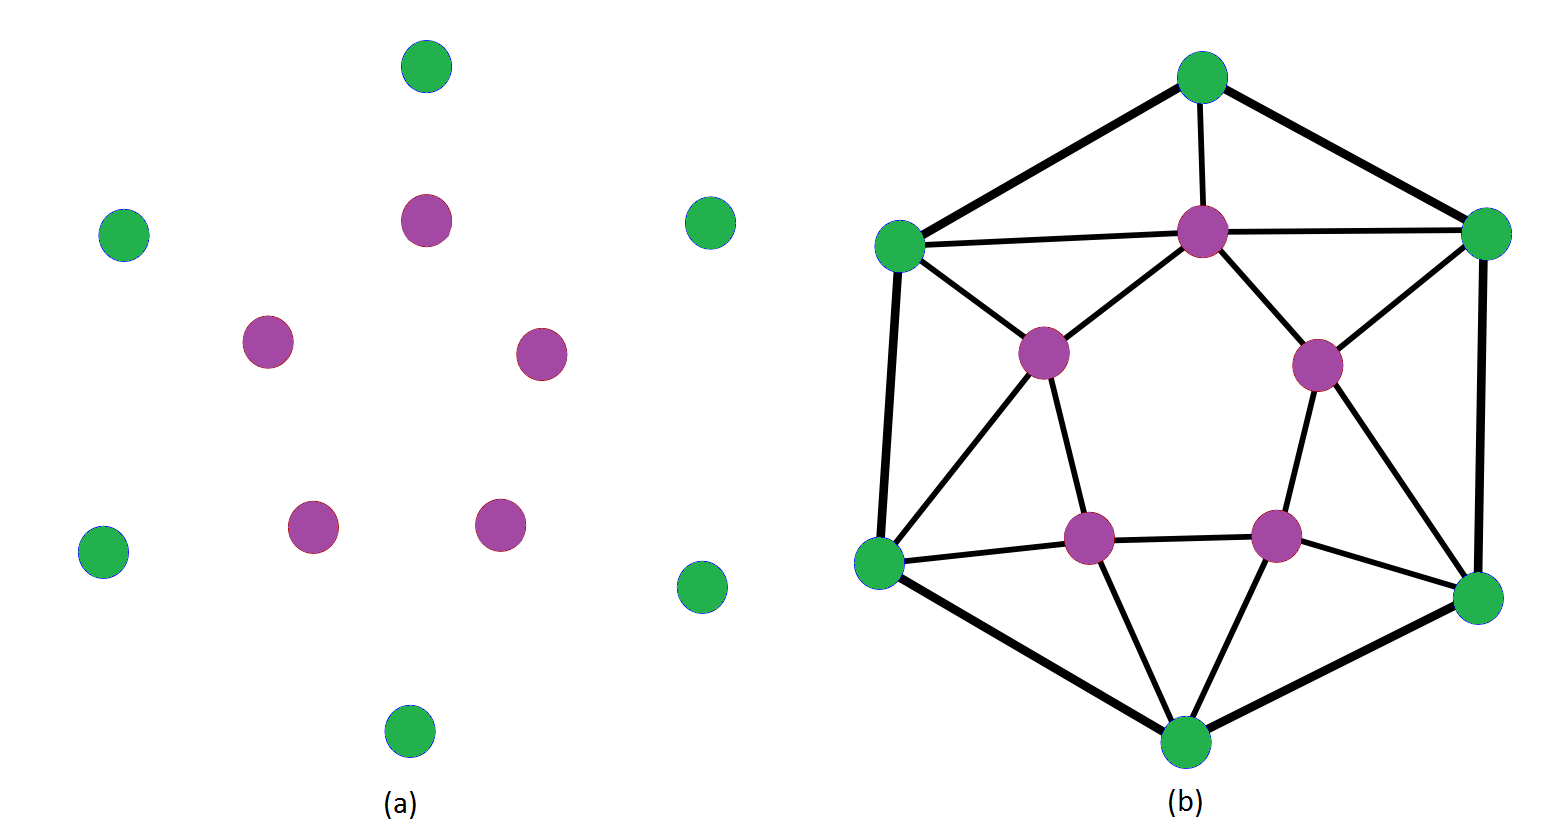
\includegraphics[width=0.7\textwidth]{images/cycle_del}
%    \caption[Delaunnay triangulation closing cyclic mesh]{Delaunnay triangulation of input points (a) used to generate faces between vertices forming the cycle (b); Green points represent vertices corresponding to cycle node 1 and violet represent vertices of cycle node 2 from Figure \ref{fig:cycle_ilu}.}
%    \label{fig:del_ilu}
%\end{figure}
%
%\begin{figure}[ht]
%    \centering
%    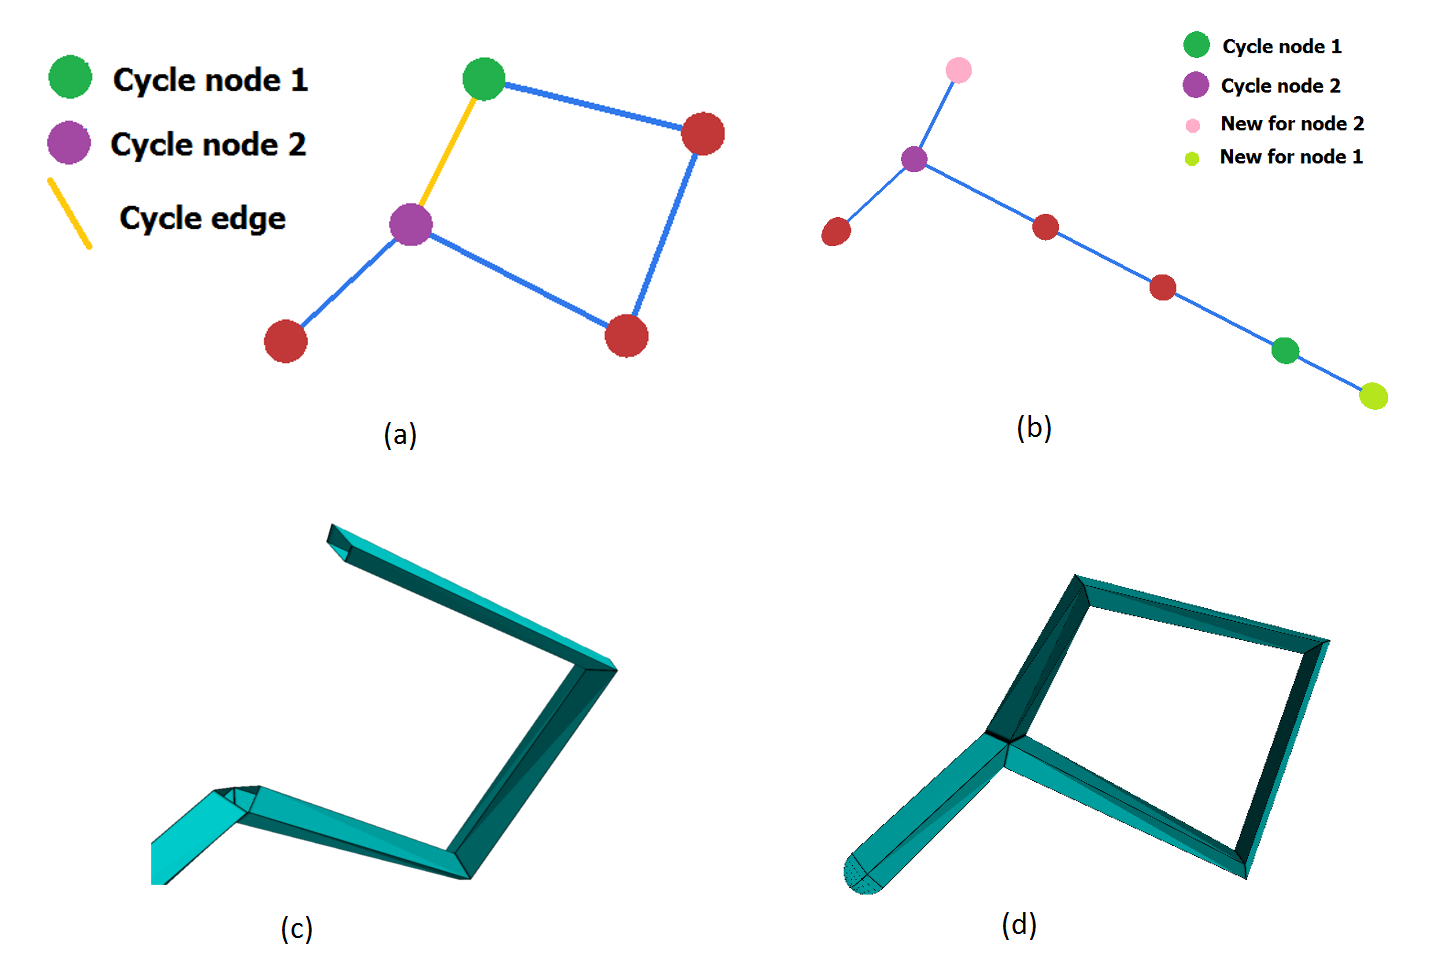
\includegraphics[width=\textwidth]{images/cyclic_skeletons}
%    \caption[Cyclic skeleton generation overview]{Cyclic skeleton base mesh generation. Cyclic skeleton, cyclic edge marked with yellow color, cyclic nodes with green and violet (a); Split cycle with one inserted node for each former cyclic nodes lightgreen for green node and pink for violet node (b); Generated base mesh before the cycle is closed (c); Generated base mesh after the cycle is closed (d).}
%    \label{fig:cycle_ilu}
%\end{figure}

\begin{figure}[ht]
        \centering
        \begin{subfigure}[b]{0.4\linewidth}
        \centering
			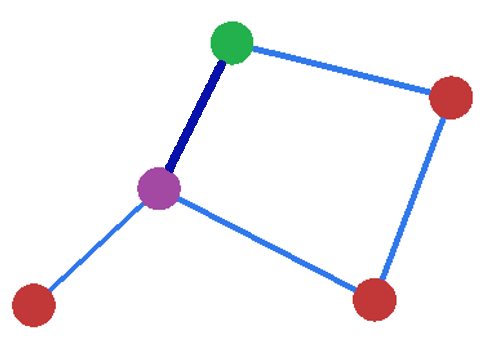
\includegraphics[width=0.9\linewidth]{images/cyclic_skeletons_1}
            \caption{Cyclic skeleton, cyclic edge marked with yellow color, cyclic nodes with green and violet}
            \label{fig:cycle_skeleton}
        \end{subfigure}%
        ~ %add desired spacing between images, e. g. ~, \quad, \qquad etc.
          %(or a blank line to force the subfigure onto a new line)
        \begin{subfigure}[b]{0.4\linewidth}
        \centering
			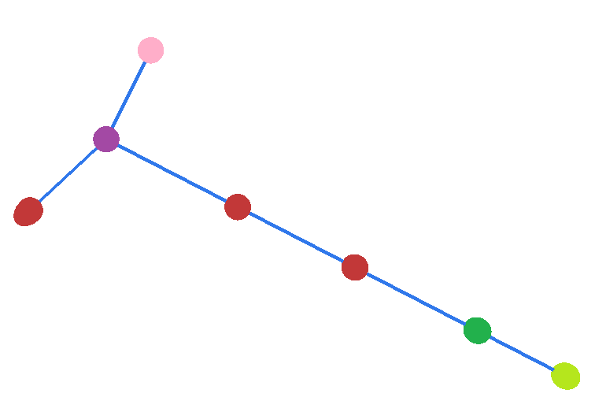
\includegraphics[width=0.9\linewidth]{images/cyclic_skeletons_2}
            \caption{Split cycle with one inserted node for each former cyclic nodes light green for green node and pink for violet node}
            \label{fig:cycle_break}
        \end{subfigure}
        \\ %add desired spacing between images, e. g. ~, \quad, \qquad etc.
          %(or a blank line to force the subfigure onto a new line)
        \begin{subfigure}[b]{0.4\linewidth}
        \centering
			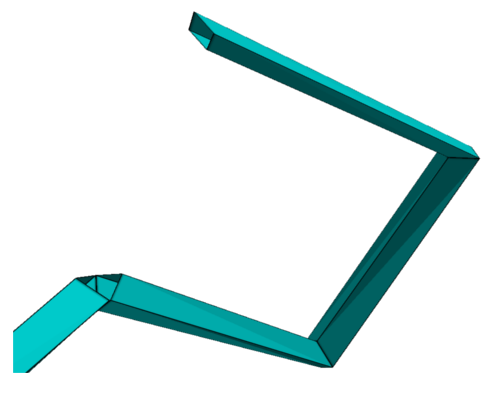
\includegraphics[width=0.9\linewidth]{images/cyclic_skeletons_3}
            \caption{Generated base mesh before the cycle is closed}
            \label{fig:cycle_before}
        \end{subfigure}
        ~ %add desired spacing between images, e. g. ~, \quad, \qquad etc.
          %(or a blank line to force the subfigure onto a new line)
        \begin{subfigure}[b]{0.4\linewidth}
        \centering
			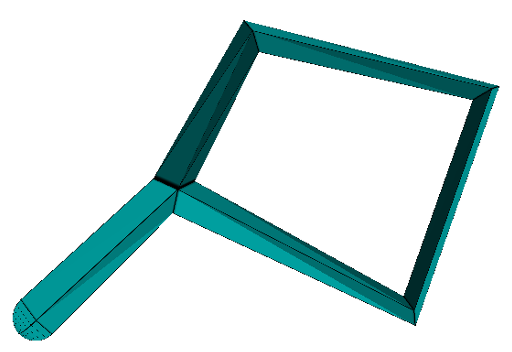
\includegraphics[width=0.9\linewidth]{images/cyclic_skeletons_4}
            \caption{Generated base mesh after the cycle is closed}
            \label{fig:cycle_after}
        \end{subfigure}
        \\ %add desired spacing between images, e. g. ~, \quad, \qquad etc.
          %(or a blank line to force the subfigure onto a new line)
        \begin{subfigure}[b]{0.4\linewidth}
        \centering
			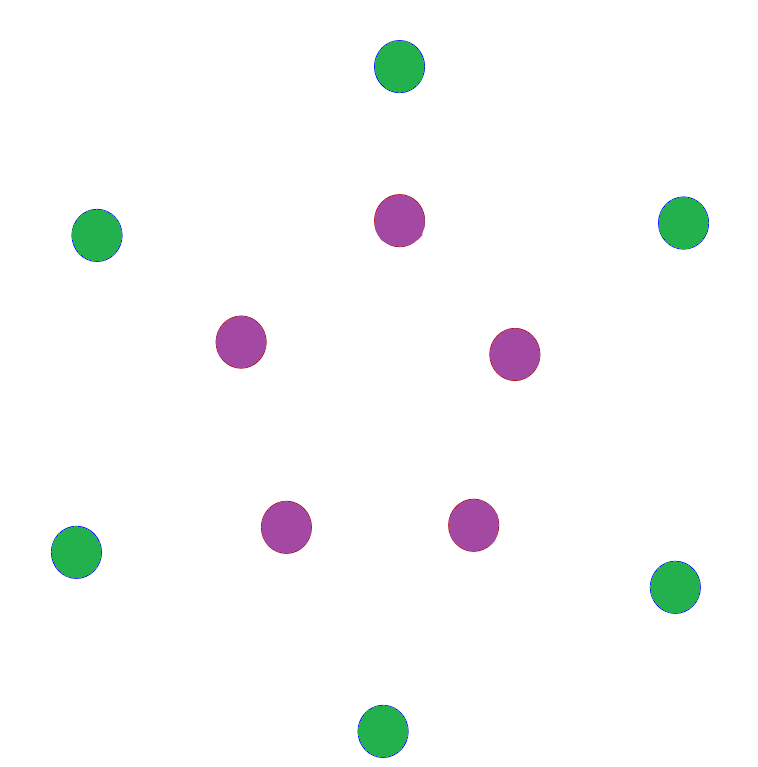
\includegraphics[width=0.8\linewidth]{images/del_tria_1}
            \caption{Vertices corresponding to green and violet cyclic nodes projected onto the same plane}
            \label{fig:cycle_del_before}
        \end{subfigure}
        ~ %add desired spacing between images, e. g. ~, \quad, \qquad etc.
          %(or a blank line to force the subfigure onto a new line)
        \begin{subfigure}[b]{0.4\linewidth}
        \centering
			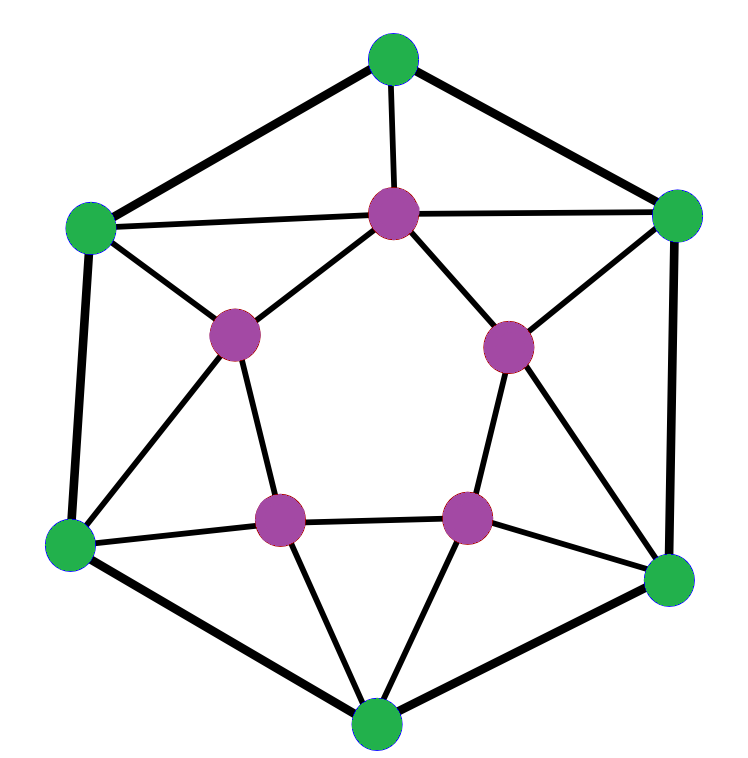
\includegraphics[width=0.8\linewidth]{images/del_tria_2}
            \caption{Faces generated by triangulation that will be used between original unprojected vertices}
            \label{fig:cycle_del_after}
        \end{subfigure}
        \caption{Cyclic skeleton base mesh generation.}
        \label{fig:cycle_ilu}
\end{figure}
